\documentclass[UTF8]{ctexart}
\usepackage{cite}
\usepackage{url}
\usepackage{amsfonts}    
\usepackage{amsmath}      
\usepackage{amssymb}
\usepackage{listings}
\usepackage{graphicx}
\usepackage{subfigure}
\usepackage{xspace}
\usepackage{float} 

\title{读书笔记(二)}
\author{黄怀宇}
\date{\today}

\lstdefinestyle{styleM}{language=matlab}
\lstdefinestyle{stylePy}{language=python}

\begin{document}
\maketitle

% \section{Abstract}
%     \subsection{方向}
%         Outlier detection, also known as anomaly detection, refers to the identification of rare items, events or observations which differ from the general distribution of a population \cite{zhao2019pyod}。在现实情况中,异常检测问题往往是没有标签的,训练数据中并未标出哪些是异常点,因此必须使用无监督学习 \cite{link1}。 因此,接下来的讨论主要放在无监督学习上。% 也就是不讨论 KNN 之类的有监督或半监督学习的算法
%     \subsection{计划}
%         主要分为三个模块,分别是情境的确定,算法的分析与测试,异常检测结果的评价。
%         \subsubsection{确定情境}
%             进度:用 sklearn 的 datasets,模拟包括网络流量(降维后)在内的其它情境。
            
%             % 第一次&第二次:尚未开始,目前用随机数据代替。% 情境用网络流量,放一到两个算法到下一篇笔记中,先搞。

%             % 第一次&第二次: 想法:可以自己爬数据,制作数据集,或用网上现成的数据集。
%         \subsubsection{无监督学习异常检测算法的分析与测试} 
%             % 第一次:进度:
%                 % 了解: Local Outlier Factor(基于相似度衡量的模型的代表算法),Isolation Forest(集成异常检测与模型融合的代表算法,通过划分子空间寻找异常点),k-means(基于极大似然估计理论的优化算法与聚类的代表算法)。
%                 % 淘汰落后的算法,例如各种基于统计与概率模型(速度快但效果不好)的算法,选择目前学术界和工业界都在用的算法,抓住主脉,其它的算法基本上都是“主脉算法”的 变形/改进/延申/组合。
%                     % 例如:
%                         % LOF 算法的延申可能表示为基于距离、夹角或是划分超平面的算法,但把数据经过类似投影之类的变换后,本质上还是基于密度的 LOF 算法。dbscan 这种基于密度的算法也是和LOF属于同一种思想的。
%                         % GMM k-means

%                 % 学习,抓住主脉算法的依据是,统一类算法适用的情境大致相似,不同主脉算法之间的差距比较大,适用的情境也就自然不同了。

%                 % 第二次:了解: PCA(线性模型的代表算法)。OneClassSVM(基于支持向量机),(SVDD、AutoEncoder)。

%                 % 第一次&第二次:可能需要了解:dbscan,  Robust Covariance,谱聚类。

%             % 第一次&第二次:想法:结合异常检测结果的评价标准,实现选择模型,性能测试的自动化。
%         \subsubsection{异常检测结果的评价}
%             % 第一次&第二次:需要了解异常检测结果的评价标准。

% \section{环境与工具说明}
%     \subsection{SKlearn}
%         scikit-learn,又写作 sklearn,是一个开源的基于 python 语言的机器学习工具包。
%         它通过 NumPy, SciPy 和 Matplotlib 等 python 数值计算的库实现高效的算法应用,并
%         且涵盖了几乎所有主流机器学习算法 \cite{link2}。 sklearn 中常用的模块有分类、回归、聚类、降维、模型选择、预处理。研究需要用到的模块主要是聚类,即:将相似对象自动分组。常用的算法有:k-Means、 spectral clustering、mean-shift,常见的应用有:客户细分,分组实验结果。
%     \subsection{Anaconda}
%         Anaconda 提供 scikit-learn 作为其免费发行的一部分
%     \subsection{PyOD}
%         PyOD is an open-source Python toolbox for performing scalable outlier detection on multi-
%         variate data \cite{zhao2019pyod}。相较于 SKlearn,拥有更多的异常检测算法与模型,在异常检测方面的专业性较之更强。

\section{算法原理与实现}
%     \subsection{k-means clustering}
%         朴素的 k-means 算法。\cite{link3}

%         Assignment step: \[ S_{i}^{(t)}={\big \{}x_{p}:{\big \|}x_{p}-m_{i}^{(t)}{\big \|}^{2}\leq {\big \|}x_{p}-m_{j}^{(t)}{\big \|}^{2}\ \forall j,1\leq j\leq k{\big \}}, \] \qquad Update step:\[ {\displaystyle m_{i}^{(t+1)}={\frac {1}{\left|S_{i}^{(t)}\right|}}\sum _{x_{j}\in S_{i}^{(t)}}x_{j}} \] 
%         \qquad 先随机生成 k 个点,当作这些 clusters 的中心,这些 clusters 的数量假设为 N, 这些中心点的个数是人为给定的。假设数据之间的相似度可以使用欧氏距离度量,即:欧氏距离越小,两个数据相似度越高。算法的步骤是先随机生成 k 个对应维度的点,% K-Means算法的特点是类别的个数是人为给定的,如果让机器自己去找类别的个数,有AP聚类算法
%         如果算法未收敛,就一直执行下面的操作:对于 N 个点,分别计算每个点属于哪一类;对于K个中心点,先找出所有属于自己这一类的所有数据点,再把自己的坐标修改为这些数据点的中心点坐标。下面使用 Matlab 的 kmeans 函数实现一下。

% \begin{lstlisting}[style=styleM]
% G1 = randn(100,2).*1+3;
% G2 = randn(100,2).*1;
% G3 = randn(100,2).*1-3;
% X = [G1;G2;G3];
% k = 3;
% cls = kmeans(X,k);
% figure(1)
% subplot(1,2,2)
% Legends = {'r.','b.','g.'};
% hold on
% for i = 1:3
%   plot(X(find(cls==i),1),X(find(cls==i),2),Legends{i})
% end
% hold off
% title('results')
% subplot(1,2,1)
% plot(X(:,1),X(:,2),'.')
% title('initial data')
% \end{lstlisting}
% \begin{figure}[ht]
% \centering
% 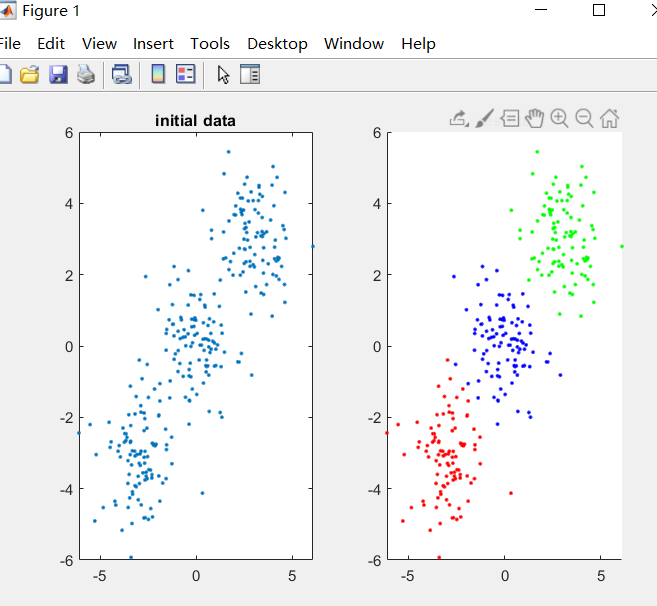
\includegraphics[scale=0.8]{kmeans_m1.png}
% \caption{k-means matlab}
% \end{figure}

%         \subsubsection{原理}
%             k-means 算法基于 Expectation-Maximization Algorithm,E 步求期望,M 步求极大。EM 算法用来解决含有 latent variable(s) 的估计问题。在 k-means 算法中,latent variables 是每个点所属的 label,用中心点给样本标注类别(或每次确认中心点以后重新进行标记)是 E 步,将中心点移动到新标的样本点的中心(或求当前分类下的中心点)是 M 步 \cite{link5}。

%             可以把 k-means 算法的 latent variables,即每个点所属类别的 label,记作 \( r_{nk} \) 矩阵,要求当前分类下的中心点,就要使给定 \( r_{nk} \) 使得损失函数最小,损失函数的形式在下文已经给出,若对其求偏导,使其偏导数等于 0:$$
%             \frac{\partial \widetilde{J}}{\partial \mu_{k}}=2 \sum_{i=1}^{N} r_{i k}\left(x_{i}-\mu_{k}\right)=0$$ 就可以每个点到中心点的指向向量的和为0:$$
%             \mu_{k}=\frac{\sum_{i=1}^{N} r_{i k} x_{i}}{\sum_{i=1}^{N} r_{i k}}$$

%         \subsubsection{初始化中心点}
%             生成数据时候以所有数据的中心点为中心,以这些数据的尺度为因子,乘以服从标准正态分布的数据。若某些中心点拿了太多点,导致其它中心点没有点拿了,算法把就需要这个点初始化到中心点附近的地方,否则在若有权重参与计算时可能出现除零错误。

%         \subsubsection{判断算法是否收敛}
%             使用代价函数(损失函数) $$\widetilde{J}=\sum_{i=1}^{C} \sum_{j=1}^{N} r_{i j} \times \nu\left(x_{j}, \mu_{i}\right)$$
            
%             \( \nu\left(x_{j}, \mu_{i}\right)=\left\|x_{j}-\mu_{i}\right\|^{2} \) 
            
%             \( r_{i j} \):若第 j 个数据点属于第 i 类,则记为 1,否则,记为 0。(大小为 \( {N} \times {C} \) 的矩阵)

%         \subsubsection{代价函数不收敛的解决办法}
%             不收敛的原因是产生了振荡,需要让中心点更新位置时参考上一次自己所在的位置,可以用阻尼比(取值在0~1之间)决定代价函数收敛的速度,在震荡不发生的情况下尽可能地使阻尼取小一点的值。\( \vec{C}^{u p d}=\vec{C}^{n e w} \times(1-\xi)+\vec{C}^{o l d} \times \xi \),其中,\( \vec{C}^{u p d} \) 是最后中心点的取值,\( \vec{C}^{n e w}\) 是当前集合的中心点, \( \vec{C}^{o l d} \) 是原来的中心点坐标。\cite{link4}

%         \subsubsection{设置权重}
%             使用加权平均值的算法 \( Mean_{weight}\left(\left\{\overrightarrow{v_{i}}\right\}, \vec{w}\right)=\sum_{i=1}^{n} w_{i} \times \overrightarrow{v_{i}} \)

%         \subsubsection{实现}
%             调用 PyOD models 中的 CBLOF 模块,里面包含了 k-means 的实现,而其实现本质上是调用了 sklearn.cluster 中的 KMeans 函数。这个 KMeans 函数经历了数十年的迭代优化,所以基本上可以把它当成是 Python 上的最优实现,而 PyOD 在这里的功能是提供生成训练数据、测试数据和可视化数据的接口,使研究人员得以更方便得调用类似 k-means 的算法,下面是我基于 PyOD 对 k-means 算法的实现测试。

% \begin{lstlisting}[style=stylePy]
% from pyod.models.cblof import CBLOF  
% from pyod.utils.data import generate_data
% from pyod.utils.example import visualize

% X_train, X_test, y_train, y_test = generate_data(n_train
%   = 2000, n_test=1000, n_features=2, behaviour="new")

% clf_name = 'CBLOF'
% clf = CBLOF()
% clf.fit(X_train)

% # binary labels (0: inliers, 1: outliers)
% y_train_pred = clf.labels_  

% # raw outlier scores
% y_train_scores = clf.decision_scores_  

% # outlier labels (0 or 1)
% y_test_pred = clf.predict(X_test)  

% # outlier scores
% y_test_scores = clf.decision_function(X_test)  

% visualize(clf_name, X_train, y_train, X_test, y_test,
%   y_train_pred, y_test_pred, show_figure=True, save_figure=False)
% \end{lstlisting}
% \begin{figure}[ht]
% \centering
% 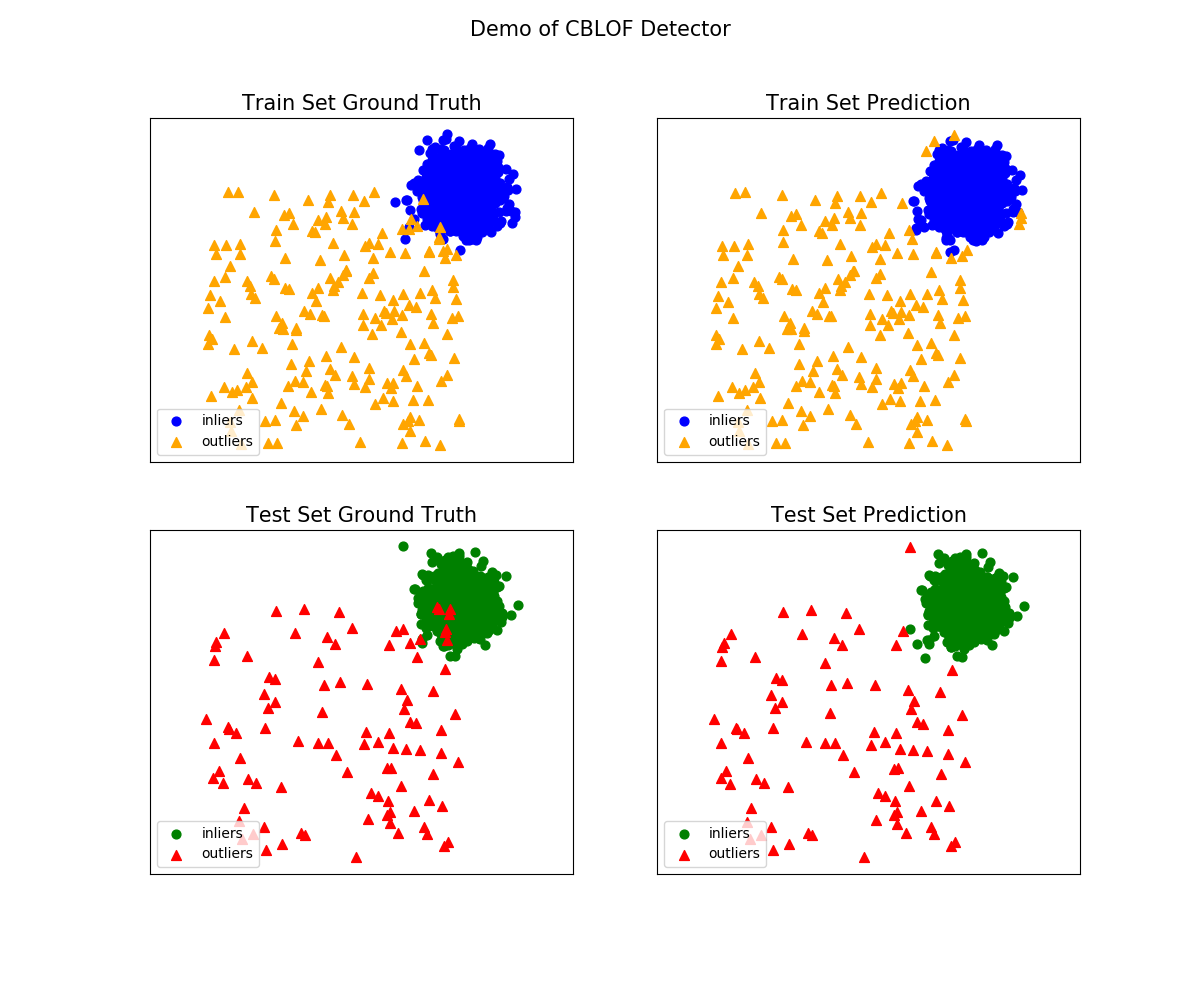
\includegraphics[scale=0.5]{kmeans_py1.png}
% \caption{k-means python}
% \end{figure}

%         \subsubsection{评价}
%             k-means 算法聚类效果较优,但可能陷入局部极小值,其结果依赖初值的位置和个数,在初始化不恰当的时候可能陷入如图 3 所示的情况。
% \begin{figure}[ht]
% \centering
% 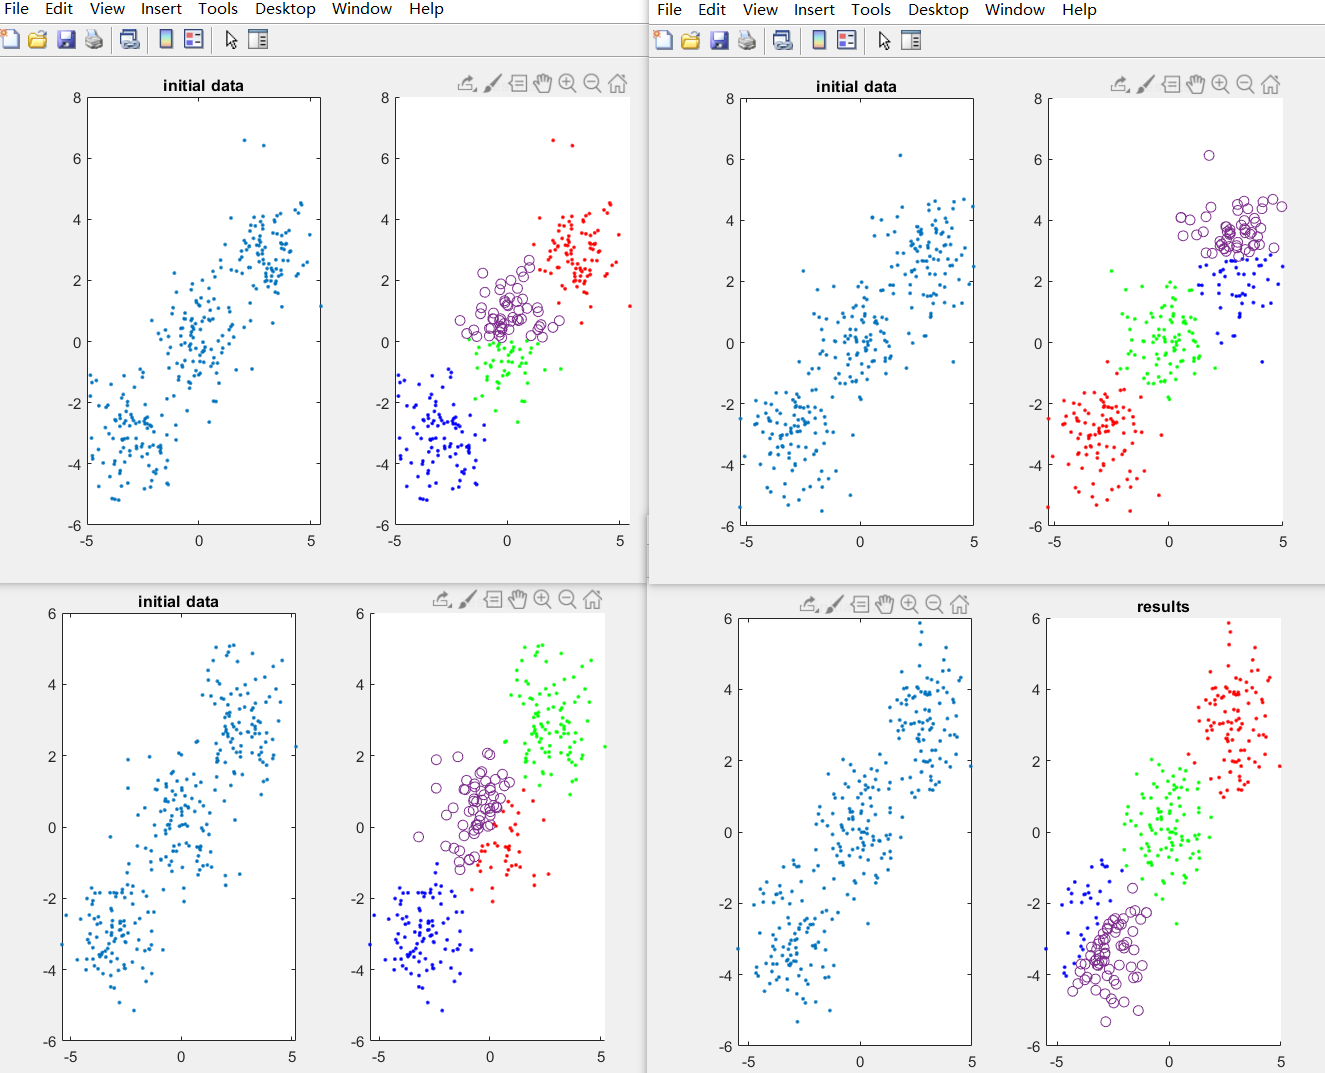
\includegraphics[scale=0.5]{kmeans_m2.png}
% \caption{k-means python}
% \end{figure}

%     \subsection{Isolation forest}
%         Isolation Forest uses a different approach: instead of trying to build a model of normal instances, it explicitly isolates anomalous points in the dataset. The main advantage of this approach is the possibility of exploiting sampling techniques to an extent that is not allowed to the profile-based methods, creating a very fast algorithm with a low memory demand. \cite{4781136} \cite{10.1145/2133360.2133363} 算法的核心思想是:对数据进行切分,比较疏离的点通过较少的次数就可以被切分出来,比较密集的点需要更多的次数才能被分出来,所以异常数据通过几次较少的切分就可以被划分出来。此算法使用的数据结构是二叉树,数据的疏离程度越深,它在二叉树的位置越浅。

%         \subsubsection{原理}
%             算法的步骤主要包含训练和预测。训练的过程是,先从全量数据中抽取一批样本,然后随机选择一个特征作为起始节点,并在该特征的最大值和最小值之间随机选择一个值,将样本中小于该取值的数据划到左分支,大于等于该取值的划到右分支。然后,在左右两个分支数据中,重复上述步骤,直到数据不可再分或二叉树达到限定的最大深度,如此这般,可构建一棵 iTree。预测的过程是,先要估算数据 x 的异常分值在每棵 iTree 中的路径长度(深度),假设 iTree 的训练样本中同样落在 x 所在叶子节点的样本数为 T.size,则数据 x 在这棵 iTree 上的路径长度 h(x),可以用下面这个公式计算:$$h(x)=e+C(T . { size })$$ 公式中,e 表示数据 x 从 iTree 的根节点到叶节点过程中经过的边的数目,C(T.size) 可以认为是一个修正值,它表示在一棵用 T.size 条样本数据构建的二叉树的平均路径长度。一般的,C(n) 的计算公式如下:$$ C(n)=2 H(n-1)-\frac{2(n-1)}{n} $$ 其中,H(n-1) 可用 ln(n-1)+0.5772156649 估算,这里的常数是欧拉常数。数据 x 最终的异常分值 Score(x) 综合了多棵 iTree 的结果:$$ S \operatorname{core}(x)=2^{-\frac{E(h(x))}{C(v)}} $$ 公式中,E(h(x)) 表示数据 x 在多棵 iTree 的路径长度的均值,[公式] 表示单棵 iTree 的训练样本的样本数,[公式] 表示用[公式]条数据构建的二叉树的平均路径长度,它在这里主要用来做归一化。从异常分值的公式看,如果数据 x 在多棵 iTree 中的平均路径长度越短,得分越接近 1,表明数据 x 越异常;如果数据 x 在多棵 iTree 中的平均路径长度越长,得分越接近 0,表示数据 x 越正常;如果数据 x 在多棵 iTree 中的平均路径长度接近整体均值,则打分会在 0.5 附近。 \cite{link6}

%         \subsubsection{实现}
%             同样的,PyOD 也是调用了 sklearn 中的 IsolationForest 算法,避免了重复造轮子。PyOD 的另一个功能是统一了各个算法的调用接口,方便了之后的 benchmark,但其部分细节需要优化,在这里,我在调用 PyOD 模块的同时,修改了 pyod.models.iforest 中构造函数的源码,把 behaviour 从 old 改成 new,其余的测试代码的编写与之前大同小异。

% \begin{lstlisting}[style=stylePy]
% from pyod.models.iforest import IForest  
% from pyod.utils.data import generate_data
% from pyod.utils.example import visualize

% X_train, X_test, y_train, y_test = generate_data(n_train=2000,
%   n_test=1000, n_features=2, behaviour="new")

% clf_name = 'IsolationForest'
% clf = IForest()
% clf.fit(X_train)

% y_train_pred = clf.labels_ 
% y_train_scores = clf.decision_scores_
% y_test_pred = clf.predict(X_test) 
% y_test_scores = clf.decision_function(X_test) 

% visualize(clf_name, X_train, y_train, X_test, y_test,
%   y_train_pred, y_test_pred, show_figure=True, save_figure=False)
% \end{lstlisting}
% \begin{figure}[ht]
% \centering
% 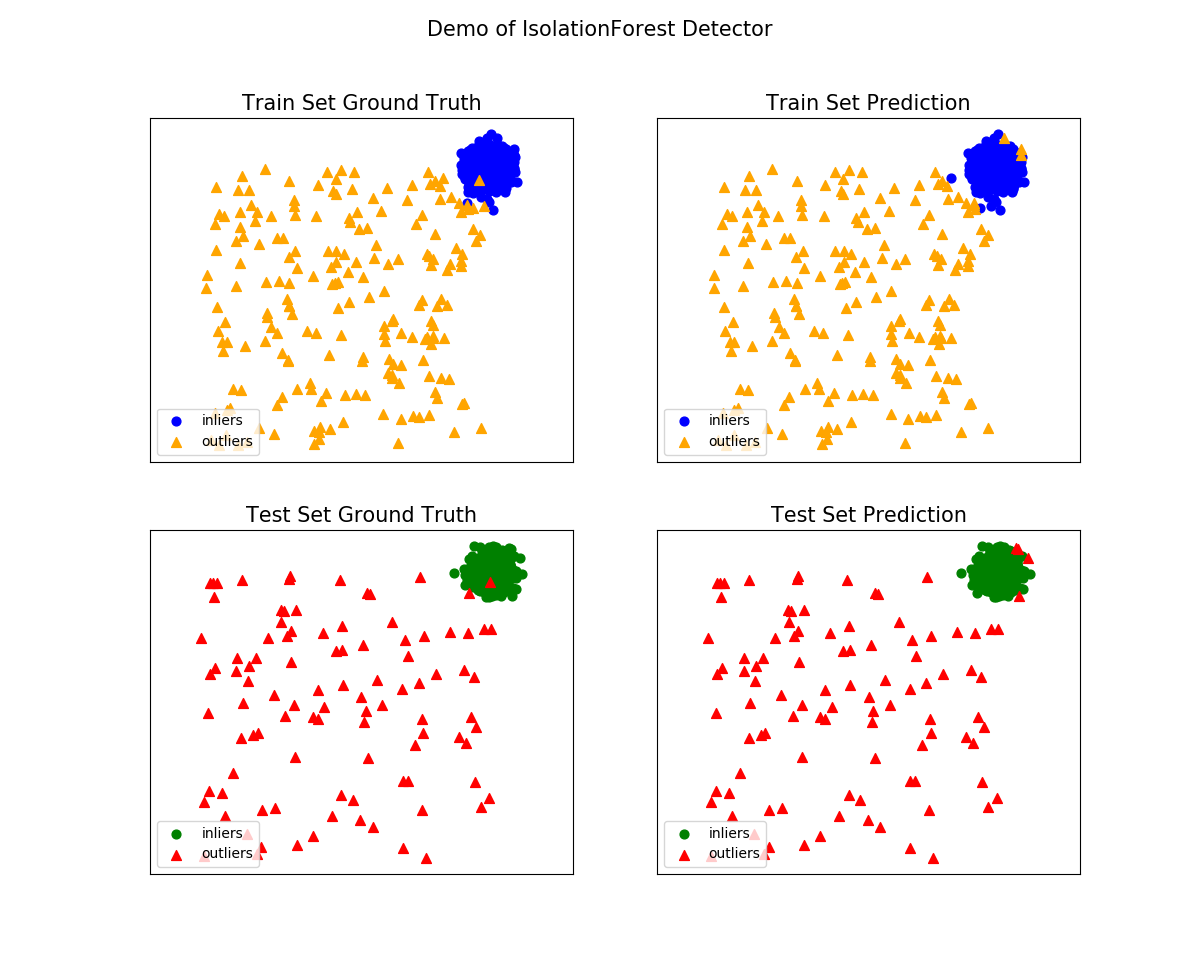
\includegraphics[scale=0.5]{IForest_py1.png}
% \caption{Isolation Forest python}
% \end{figure}

%         \subsubsection{评价}
%             此算法速度快,但若训练样本中异常样本的比例较高,可能影响算法最终的效果;算法检测出的“异常”在实际应用情景中不一定是实际想要的异常。

%     \subsection{Local Outlier Factor}
%         LOF 是基于密度的算法,核心是表示和描述数据点的密度。

%         \subsubsection{k-distance}
%             K-邻近距离:第 k 个最近的距离数据点 p 的距离。

%         \subsubsection{rechability distance}
%             可达距离:给定数据点 p 和 o,其中,o 的 k-distance 已知, p 到 o 的可达距离为 o 的 K-邻近距离 和 p 与 o 之间的直接距离的最大值。 $$ \operatorname {reach\_dist}_{k}(p, o)=\max \{k-\operatorname {distance}(o), d(p, o)\} $$

%         \subsubsection{local rechability density}
%             局部可达密度:计算的是绝对局部密度,对于数据点 p,那些跟 p 的距离小于等于 k-distance(p)的数据点称为它的 k-nearest-neighbor,记为 $N_k(p)$,数据点 p 的局部可达密度为它与邻近的数据点的平均可达距离的倒数。 $$ lrd_{k}(p)=\frac{1}{\frac{\sum_{o\in{N_{k}(p)}}reach\_dist_k(p,o)}{|N_k(p)|}} $$

%         \subsubsection{local outlier factor}
%             局部异常因子:计算的是数据点 p 跟周围邻近的数据点的相对密度,好处是可以允许数据出现分布不均匀、密度不同的情况,p 的局部异常因子是 p 的邻居们的平均局部可达密度跟数据点p的局部可达密度的比值。$$ LOF_{k}(p)=\frac{\sum_{o\in{N_k(p)}}\frac{lrd(o)}{lrd(p)}}{|N_{k}(p)|}=\frac{\sum_{o\in{N_{k}(p)}}lrd(o)}{|N_{k}(p)|}/lrd(p) $$

%         \subsubsection{原理}
%             根据 LOF 的 定义计算出 LOF(k) 后:LOF(k) ~ 1 表示与 neighbors 密度相似,LOF(k) < 1 表示密度大于 neighbors (Inlier),LOF(k) > 1 表示密度低于 neighbors (Outlier)

%         \subsubsection{实现}
%             还是用 PyOD 的模块实现,代码与之前的大同小异。它还是调用了 sklearn 的 LocalOutlierFactor 算法,不重复造轮子。

% \begin{lstlisting}[style=stylePy]
% from pyod.models.lof import LOF  
% from pyod.utils.data import generate_data
% from pyod.utils.example import visualize

% X_train, X_test, y_train, y_test = generate_data(n_train=2000, n_test=1000, n_features=2, behaviour="new")

% clf_name = 'LOF'
% clf = LOF()
% clf.fit(X_train)

% y_train_pred = clf.labels_ 
% y_train_scores = clf.decision_scores_
% y_test_pred = clf.predict(X_test) 
% y_test_scores = clf.decision_function(X_test) 

% visualize(clf_name, X_train, y_train, X_test, y_test, y_train_pred, y_test_pred, show_figure=True, save_figure=False)
% \end{lstlisting}

% \begin{figure}[htbp]
% \centering
% \subfigure[result 1]{
% 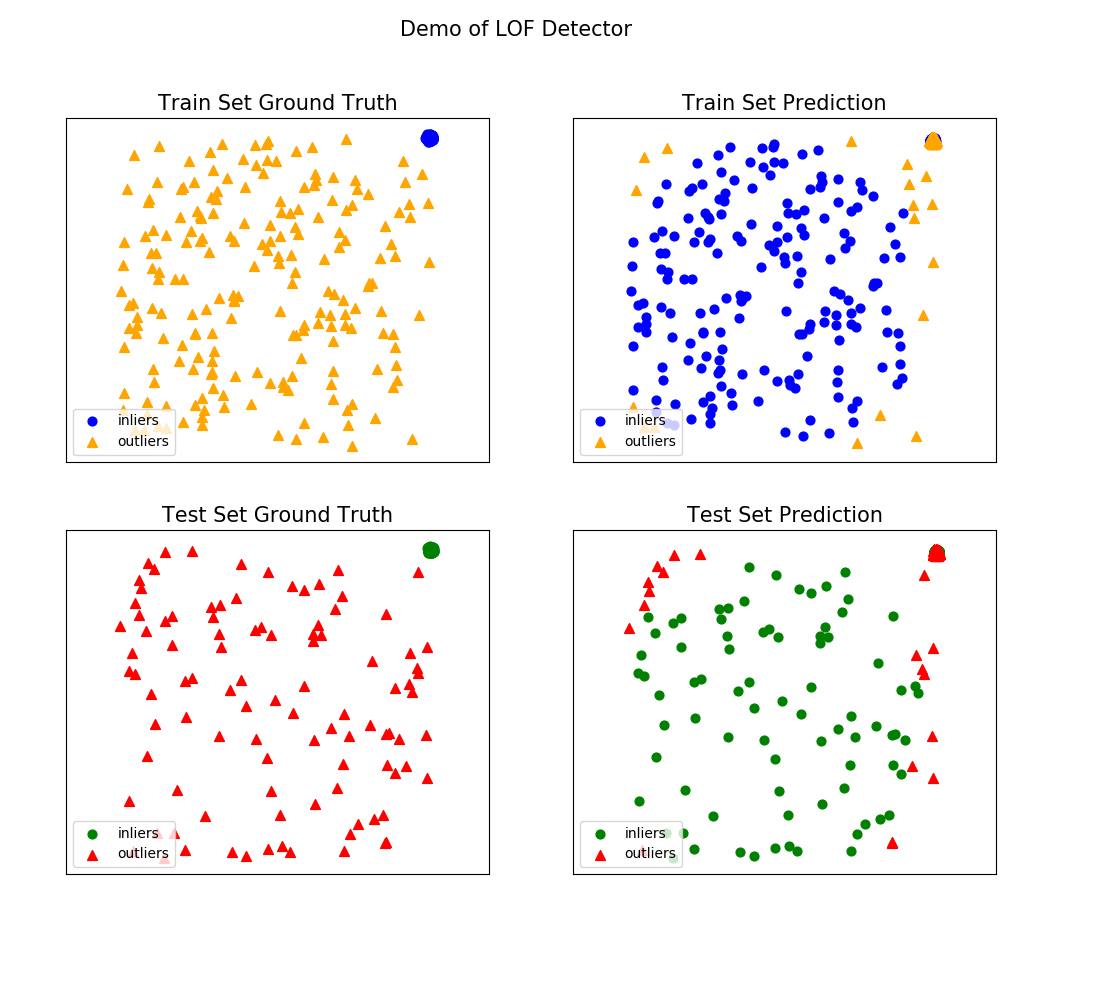
\includegraphics[width=5.5cm]{lof_py1.png}
% }
% \quad
% \subfigure[result 2]{
% 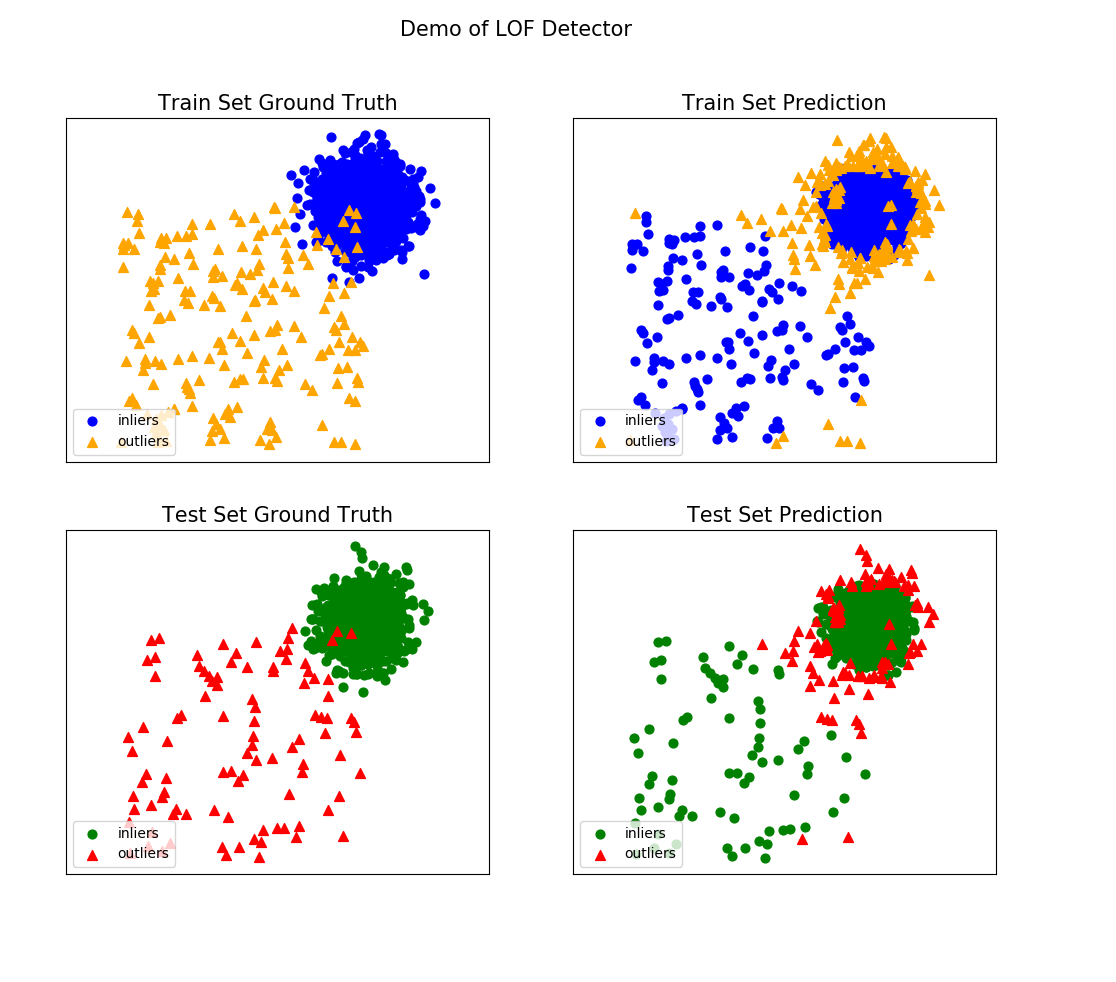
\includegraphics[width=5.5cm]{lof_py2.png}
% }
% \quad
% \subfigure[result 3]{
% 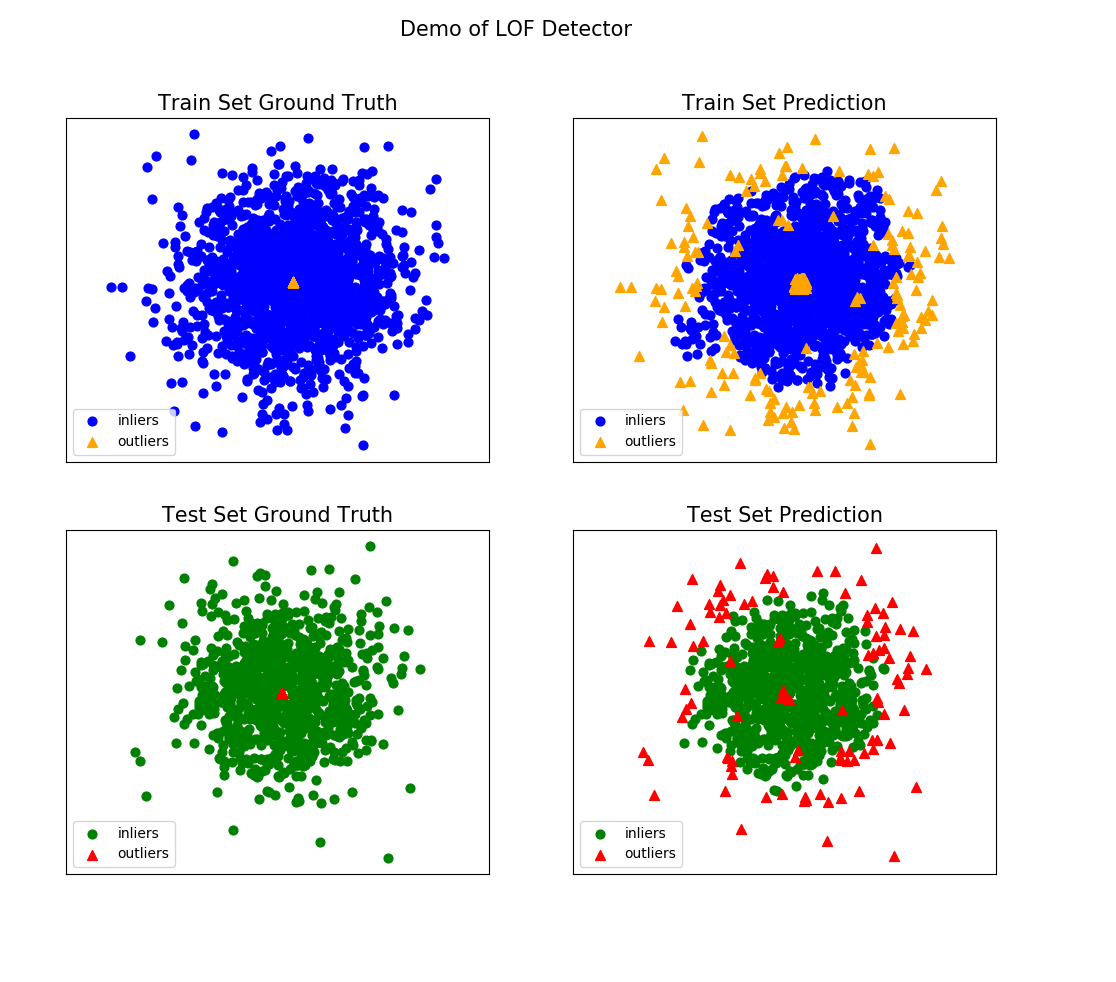
\includegraphics[width=5.5cm]{lof_py3.png}
% }
% \quad
% \subfigure[result 4]{
% 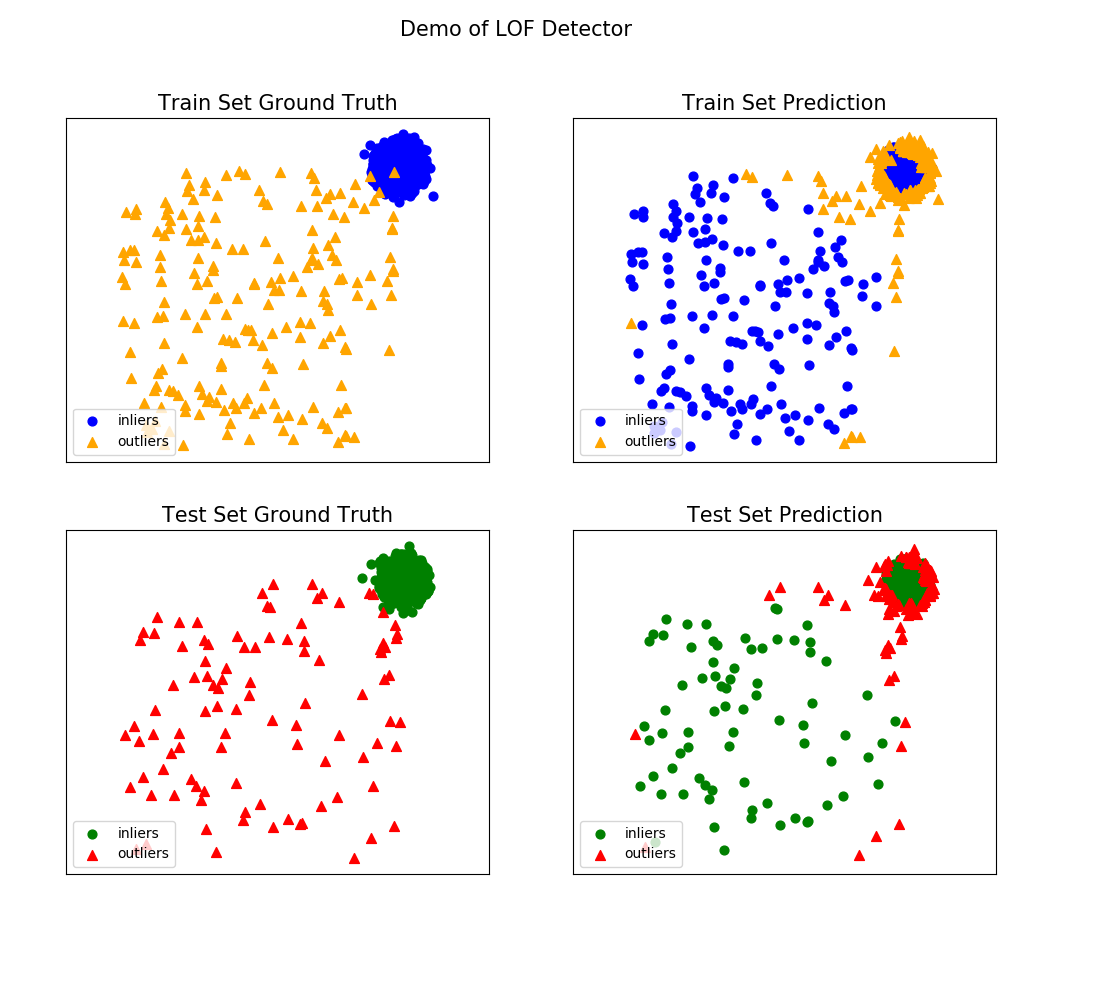
\includegraphics[width=5.5cm]{lof_py4.png}
% }
% \caption{ Local Outlier Factor}
% \end{figure}

%         \subsubsection{评价}
%             可以明显看出,这个算法与前两个算法之间的结果差异。前两个算法从直观的角度出发,是“从外向内”聚类, 类似于在异常数据与正常数据之间划了几条线进行划分,k-means 虽然有中心点,但本质上仍是数据点的站队问题,类似于多党制国家中党派之间的互相争夺选民;EM 是以不断剔除异己的方式,越到迭代的后面,剩余点的“忠诚度”就越高,类似于列宁主义;而 LOF 这种基于密度的算法则是“自内向外”扩展,好像一个个“菌落”的扩大,类似于社会上关系紧密的人自发形成社团组织。不同的算法适用于不同的情境,要充分考虑到这些算法的特点与情境的特点,灵活地选择最适合当前情境的算法或其组合。

%%%%%%%%%%%%%%%%%%%%%%%%%%%%%%%%% 第二次 %%%%%%%%%%%%%%%%%%%%%%%%%%%%%%%%%%%%%%
%%% 鉴于第一次读书笔记的测试代码的耦合性较高,之后统一用字典迭代测试 %%%
    \subsection{Principal Component Analysis}
%维度压缩(dimension reduction)     
    此算法是常见的数据降维方法,对原数据进行线性变换,并且找出信息量大的 Principal Component,去除非 Principal Component(相当于异常检测中的 anomaly/outlier)。
        \subsubsection{原理}
        首先,对原始数据进行中心化和归一化,分别使之后的公式描述更简洁,不同变量的方差变化尺度控制在相同的范围内。假设原始数据是一个 \( m \times n\) 的矩阵,m 表示数据样本的数量,n 表示每一条数据样本的特征数目。将预处理之后的矩阵表示为 \(X\),则 PCA 的主要步骤如下:

        1. 计算协方差矩阵 \(C=\frac{1}{m-1} X^{T} X\)
        
        2. 求解协方差矩阵的特征值 \(\lambda_{1}, \lambda_{2}, \ldots, \lambda_{i}\) 和特征向量 \(\mathbf{e}_{1}, \mathbf{e}_{2}, \ldots, \mathbf{e}_{\mathbf{i}}\)

        3. 按照特征值从大到小的顺序,将特征向量从左至右排列,将前k个特征向量组成的矩阵表示为 \(P_{k}\)

        4. 将 \(X\) 映射到低维的 k 维空间( \(k \ll n\) ),则映射之后的数据 \(Y_{k}=X P_{k}\)

        然后,我们要把 PCA 用于异常检测,如果把所有数据样本的重构用矩阵的形式表示出来,则得到重构公式:\(X^{\prime}=Y_{k} P_{k}^{T}\)  。对于某一个特征向量 \(\mathbf{e}_{\mathbf{j}}\),数据样本 \(x_{i}\) 在该方向上的偏离程度 \(d_{ij}\) 可以用\(d_{i j}=\frac{\left(\mathbf{x}_{\mathbf{i}}^{\mathbf{T}} \cdot \mathbf{e}_{\mathbf{j}}\right)^{2}}{\lambda_{j}}\)计算:
        这里的 \(\lambda_{j}\) 主要起归一化的作用,这样可以使得不同方向上的偏离程度具有可比性。在计算了数据样本在所有方向上的偏离程度之后,为了给出一个综合的异常得分,最自然的做法是将样本在所有方向上的偏离程度加起来,即:\(S c o r e\left(\mathbf{x}_{\mathbf{i}}\right)=\sum_{j=1}^{n} d_{i j}=\sum_{j=1}^{n} \frac{\left(\mathbf{x}_{\mathbf{i}}^{\mathbf{T}} \cdot \mathbf{e}_{\mathbf{j}}\right)^{2}}{\lambda_{j}}\) 。这个公式只是计算异常得分的一种方式。也有一些算法采取了略微不同的做法,比如,有的只考虑数据在前 k 个特征向量方向上的偏差,或者只考虑后 r 个特征向量方向上的偏差,即:\(\sum_{j=1}^{k} d_{i j}>C_{1} \quad\) or \(\quad \sum_{j=n-r+1}^{n} d_{i j}>C_{2}\) 。这里的 \(C_{1}\) 和 \(C_{2}\) 是人为设定的两个阈值,如果得分大于阈值则判断为异常。
        
        一般而言,前几个特征向量往往直接对应原始数据里的某几个特征,在前几个特征向量方向上偏差比较大的数据样本,往往就是在原始数据中那几个特征上的极值点。而后几个特征向量有些不同,它们通常表示某几个原始特征的线性组合,线性组合之后的方差比较小反应了这几个特征之间的某种关系。在后几个特征方向上偏差比较大的数据样本,表示它在原始数据里对应的那几个特征上出现了与预计不太一致的情况。到底是考虑全部特征方向上的偏差,前几个特征向量上的偏差,还是后几个特征向量上的偏差,在具体使用时可以根据具体数据灵活处理。
        
        前面提到,PCA用于异常检测时候,还有一种思路是基于重构误差的。直观上理解,PCA提取了数据的主要特征,如果一个数据样本不容易被重构出来,表示这个数据样本的特征跟整体数据样本的特征不一致,那么它显然就是一个异常的样本。对于数据样本 \(x_{i}\) , 假设其基于 k 维特征向量重构的样本为 \(\mathbf{x}_{\mathrm{ik}}^{\prime}\) , 则该数据样本的异常得分可以用如下的公式计算:
        $$
        \begin{array}{l}
        \operatorname { Score }\left(x_{i}\right)=\sum_{k=1}^{n}\left(\left|\mathbf{x}_{\mathbf{i}}-\mathbf{x}_{\mathbf{i k}}^{\prime}\right|\right) \times e v(k) \\
        e v(k)=\frac{\sum_{j=1}^{k} \lambda_{j}}{\sum_{j=1}^{n} \lambda_{j}}
        \end{array}
        $$
        上面的公式考虑了重构使用的特征向量的个数 k 的影响,将 k 的所有可能做了一个加权求和,得出了一个综合的异常得分。\cite{link7}

        \subsubsection{评价}
        此算法在降维的同时做了异常检测,可以用于可视化高维数据,辅助于人工检测。

    \subsection{One Class Support Vector Machine}
        \subsubsection{原理}
            寻找一个超平面将样本中的正例圈出来。这里选择 SVDD(Support Vector Data Description by Tax and Duin),用一个球体而不是平面来把正样例圈出来。
            
            设超球体的中心为 a,半径 R > 0,体积 \( R^{2} \) 被最小化,中心 a 是支持向量的线性组合;要求所有到数据点 \( x_{i}\) 中心的距离严格小于 R,同时构造一个惩罚系数为 C 的松弛变量 \( \zeta_{i}\),优化问题如下:

            $$
            \begin{array}{c}
            \min _{R, a} R^{2}+C \sum_{i=1}^{n} \zeta_{i} \\
            \text {s.t. }\left\|x_{i}-a\right\|^{2} \leq R^{2}+\zeta_{i}, i=1, \ldots, n \\
            \zeta_{i} \geq 0, i=1, \ldots, n
            \end{array}
            $$

            在采用拉格朗日算子求解之后,可以判断新的数据点 z 是否在类内,如果z到中心的距离小于或者等于半径。采用 Gaussian Kernel 做为两个数据点的距离函数:
            
            $$
            \|z-x\|^{2}=\sum_{i=1}^{n} a_{i} \exp \left(\frac{-\left\|z-x_{i}\right\|^{2}}{\sigma^{2}}\right) \geq-R^{2} / 2+C_{R}
            $$
            \cite{link9}
        \subsubsection{评价}
            核函数计算比较耗时,在海量数据的场景用的不多,适合数据量较小且只检测两类的情境下用。
    \subsection{统一实现}
\begin{lstlisting}[style=stylePy]
from pyod.utils.data import generate_data, 
 get_outliers_inliers
from pyod.utils.example import visualize
import numpy as np
from scipy import stats
import matplotlib.pyplot as plt
import matplotlib.font_manager

from pyod.models.iforest import IForest  
from pyod.models.abod import ABOD
from pyod.models.lof import LOF
from pyod.models.cblof import CBLOF
from pyod.models.iforest import IForest 
from pyod.models.pca import PCA 
from pyod.models.ocsvm import OCSVM

data_size = 300
outlier_fraction = 0.1

X_train, Y_train = generate_data(n_train=data_size, 
 train_only=True, n_features=2, behaviour="new")
x_outliers, x_inliers = get_outliers_inliers
 (X_train,Y_train)
n_inliers = len(x_inliers)
n_outliers = len(x_outliers)
F1 = X_train[:,[0]].reshape(-1,1)
F2 = X_train[:,[1]].reshape(-1,1)
xx , yy = np.meshgrid(np.linspace(-10, 10, data_size), 
 np.linspace(-10, 10, data_size))
plt.scatter(F1,F2)
plt.xlabel('F1')
plt.ylabel('F2') 

classifiers = {
        'k-means clustering' : CBLOF
         (contamination=outlier_fraction),
        'Isolation forest': IForest
         (contamination=outlier_fraction),
        'Local Outlier Factor' : LOF
         (contamination=outlier_fraction),
        'Principal component analysis' : PCA
         (contamination=outlier_fraction),
        'One Class Support Vector Machine' : OCSVM
         (contamination=outlier_fraction)
}

class_nums = len(classifiers)
plt.figure(figsize=(10, 10))

for i, (clf_name,clf) in enumerate
 (classifiers.items()) :clf.fit(X_train)

    # predict raw anomaly score
    scores_pred = clf.decision_function(X_train)*-1

    # prediction of a datapoint category outlier
    # or inliery_pred = clf.predict(X_train)

    n_inliers = len(y_pred) - np.count_nonzero(y_pred)
    n_outliers = np.count_nonzero(y_pred == 1)

    print('Algorithm: ', clf_name, '    OUTLIERS: ',
     n_outliers, '  INLIERS: ',n_inliers)

    # visualize
    threshold = stats.scoreatpercentile
     (scores_pred,100 *outlier_fraction)
    Z = clf.decision_function
     (np.c_[xx.ravel(), yy.ravel()]) * -1
    Z = Z.reshape(xx.shape)
    subplot = plt.subplot(1, class_nums, i + 1)
    subplot.contourf(xx, yy, Z, levels = np.linspace
     (Z.min(), threshold, 10),cmap=plt.cm.Blues_r)
    a = subplot.contour(xx, yy, Z,
     levels=[threshold],linewidths=2, colors='red')
    subplot.contourf(xx, yy, Z,
     levels=[threshold, Z.max()],colors='orange')
    b = subplot.scatter(X_train[:-n_outliers, 0],
     X_train[:-n_outliers, 1],
     c='white',s=20, edgecolor='k') 
    c = subplot.scatter(X_train[-n_outliers:, 0],
     X_train[-n_outliers:, 1],
     c='black',s=20, edgecolor='k')
    subplot.axis('tight')
    subplot.legend(
        [a.collections[0], b, c],
        ['learned decision function', 'true inliers',
         'true outliers'],
        prop=matplotlib.font_manager
         .FontProperties(size=10),
        loc='lower right')
    subplot.set_title(clf_name)
    subplot.set_xlim((-10, 10))
    subplot.set_ylim((-10, 10))
plt.show() 
\end{lstlisting}

\begin{figure}[H] %H为当前位置,!htb为忽略美学标准,htbp为浮动图形
\centering %图片居中
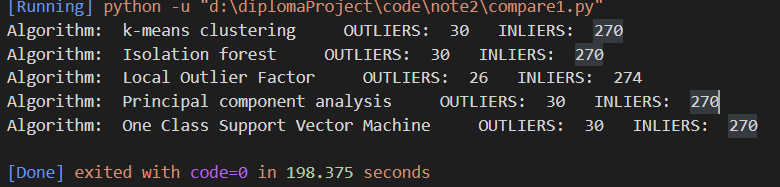
\includegraphics[width=1.1\textwidth]{plt_t1_5.png} %插入图片,[]中设置图片大小,{}中是图片文件名
\caption{Accuracy} %最终文档中希望显示的图片标题
% \label{Fig.main2} %用于文内引用的标签
\end{figure}


\begin{figure}[H]
\centering  %图片全局居中
\subfigure[Algorithm1]{
% \label{}
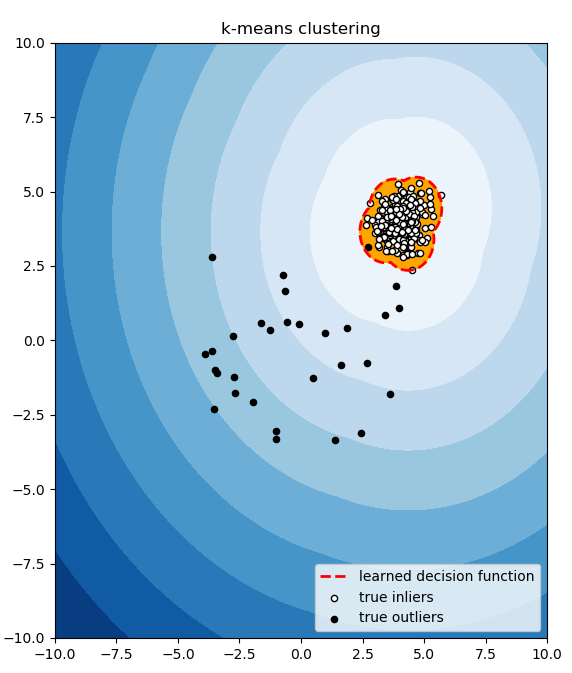
\includegraphics[width=0.45\textwidth]{plt1.png}}
\subfigure[Algorithm2]{
% \label{}
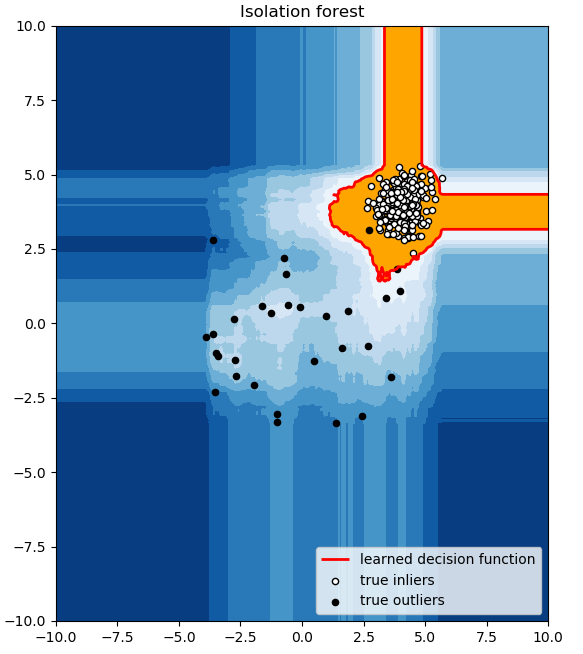
\includegraphics[width=0.45\textwidth]{plt2.png}}
\subfigure[Algorithm3]{
% \label{}
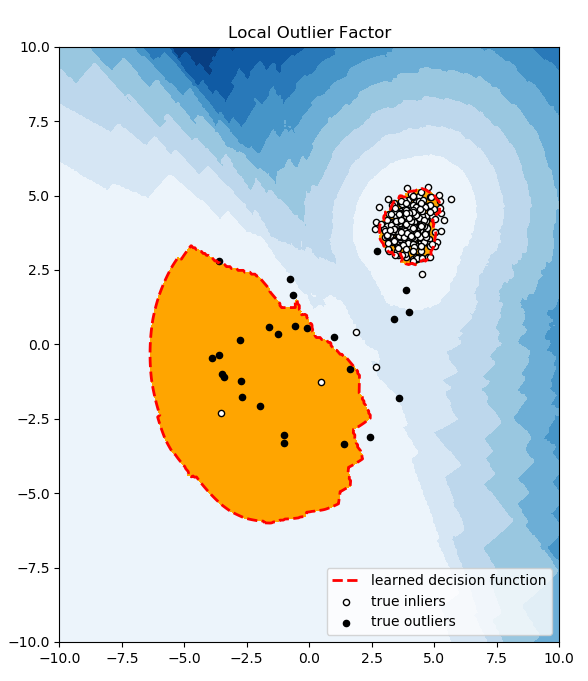
\includegraphics[width=0.45\textwidth]{plt3.png}}
\subfigure[Algorithm4]{
% \label{}
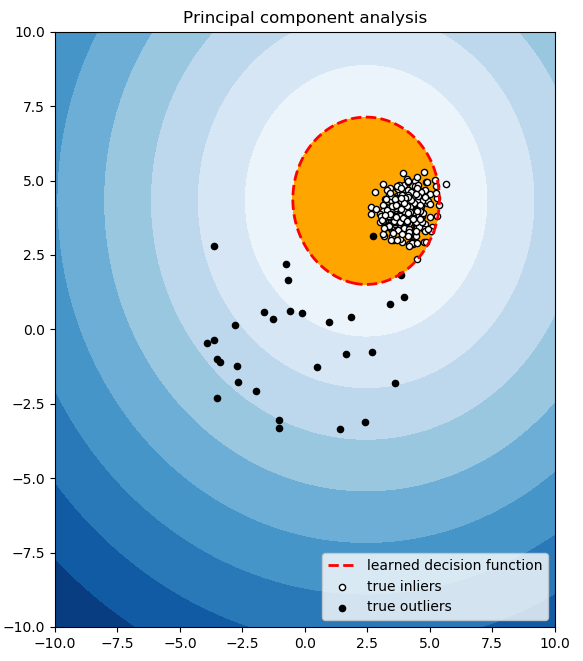
\includegraphics[width=0.45\textwidth]{plt4.png}}
\subfigure[Algorithm5]{
% \label{}
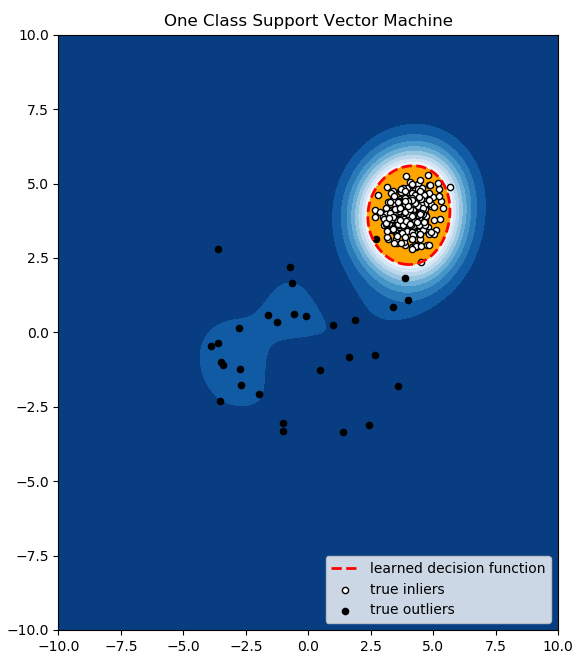
\includegraphics[width=0.45\textwidth]{plt5.png}}
\caption{Tested Algorithm}
% \label{Fig.main}
\end{figure}

可以发现在精度方面基准测试的结果可以和如下论文的结果一致,结论是:基于 LOF 的异常检测算法的精确度最高,速度适中,综合性能较其它算法更好。

\begin{figure}[H] %H为当前位置,!htb为忽略美学标准,htbp为浮动图形
\centering %图片居中
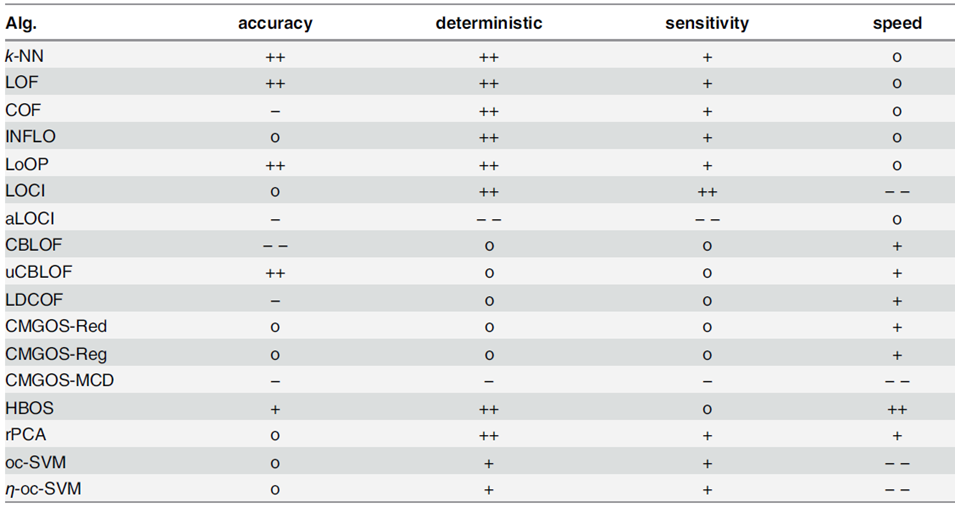
\includegraphics[width=1.0\textwidth]{cite_benchmark1.png} %插入图片,[]中设置图片大小,{}中是图片文件名
\caption{Fully benchmark} %最终文档中希望显示的图片标题
\protect\cite{Goldstein2016ACE}
% \label{Fig.main2} %用于文内引用的标签
\end{figure}
    
\section{其它算法分类与概述}
\subsection{选择无监督算法的必要性}
监控视频异常检测主要面临以下挑战:1)异常事件定义的模糊性。正常样本与异常样本之间没有明确的划分边界。2)异常事件定义的场景依赖性。同一事件在不同的场景下具有不同的异常属性。3)异常事件的稀少性、多样性、不可穷举性。4)训练样本中包含噪声, 给样本信息带来干扰。5)由于数据的隐私性,目前可用的公开数据集较少。异常样本的稀少性、不可穷举性限制了有监督算法在该领域的应用,所以选择的算法以无监督为主。\cite{qh2020}
\subsection{算法分类与概述}
\subsubsection{传统机器学习方法}
1. 点模型:

聚类判别算法首先将正常样本聚类,然后将测试集中远离聚类中心的点、属于小聚类的点判断为异常。常用的聚类算法有:k-means、k-medoids、模糊c-means、Gauss混合模型(Gaussian mixed model, GMM)。常用的判断异常的方式有:测试样本到聚类中心的距离、一类支持向量机(one-class support vector machine, OC-SVM)、k最近邻(k-nearest neighbors, KNN)与核密度估计(kernel density estimation, KDE)。

共发判别算法主要基于主题模型检测异常。算法首先将正常样本划分为若干主题,然后将不属于任何正常主题的样本判断为异常。常用的主题模型算法是隐Dirichlet分配(latent Dirichlet allocation, LDA)与层次Dirichlet过程(hierarchical Dirichlet processes, HDP)。分别使用不同的特征结合LDA检测异常。HDP常与其他模型复合使用。

在传统机器学习方法中,基于重构判别的算法主要有两种:主成分分析(principal components analysis, PCA)法与SC法。它们的思路是:正常样本存在公共因子,使得正常样本可由这些公共因子重构,而异常样本则不能。从特征空间的角度看,它们都是用低维子空间来拟合正常样本在特征空间的分布。不同的是,PCA法用一个单一的低维子空间描述正常样本的分布,SC法通过一个过完备的字典与稀疏约束,用多个低维子空间的并集描述正常样本的分布。

2. 序列模型

在传统机器学习方法中,用于异常检测的序列模型主要是MDT与HMM,它们的判别都是生成概率判别。主要相关文献及算法如下:

MDT算法由K个线性动态系统(linear dynamic system, LDS)组成,用以捕捉正常样本的K种特征转移规律,当测试样本不符合其中任何一个特征转移规律时,将其判断为异常。

用无限HMM(infinite HMM, iHMM)模型结合Markov链Monte Carlo(Markov chain Monte Carlo, MCMC)采样或者变分Bayes公式来检测异常。用多观测HMM(multi-observation HMM, MOHMM)算法检测异常。将多个时空近邻的HMM进行耦合,构建耦合HMM(coupled HMM, CHMM),使算法结合了更多的时空关联信息。将多个HMM集成检测异常。

3. 图模型

图模型算法利用时空块之间的关联关系检测异常。图推断判别算法主要利用Markov随机场(Markov random field, MRF)检测异常。提取视频时空块的混合概率PCA(mixture of probabilistic PCA, MPPCA)特征构建MRF模型,然后基于节点与节点间的推断关系检测异常。

图结构判别将图的拓扑结构作为一种新的特征检测异常。将时空近邻的特征点相连接构建图结构,然后将图的拓扑结构映射到低维流形中,在低维流形中检测异常。用视频中时空近邻的兴趣点构建图结构,以图的拓扑结构作为新的特征,通过构建图结构相似性算子实现图结构的聚类从而检测异常。

4. 复合模型

传统机器学习方法中的复合模型主要是将点模型与序列模型结合,使算法既能检测样本的分布异常,又能检测样本的转移规律异常。将LDA与HMM结合,将HDP与HMM、OC-SVM结合,将HDP与Gauss过程(Gaussian process, GP)、HMM算法结合,将SVM与HMM结合。

\subsubsection{混合方法}

深度特征比手工特征具有更强的描述能力。在混合方法阶段,算法使用深度特征代替手工特征,然后用传统机器学习方法检测异常。在该发展阶段,得到发展的模型主要是点模型,应用的判别主要是聚类判别、重构判别和其他判别。

\subsubsection{深度学习方法}
在深度学习方法阶段,算法将特征提取步骤与模型训练步骤结合到一起,用端到端的方法检测异常。

1. 点模型

深度学习方法中的聚类算法主要有:自组织映射(self-organizing map, SOM)、生长的神经气(growing neural gas, GNG)、Gauss混合全卷积VAE(Gaussian mixture fully convolutional VAE, GMFC-VAE)、一类神经网络(one-class neural network, OC-NN)。其中:SOM、GNG通过训练将不同样本映射到不同聚类实现端到端的聚类;GMFC-VAE通过变分的方式,用GMM拟合特征空间的分布;OC-NN是一种针对异常检测的神经网络,该算法将正常样本映射到一个超球体内、异常样本映射到超球体外,通过不断收缩超球体来增强网络的异常检测能力。

2. 序列模型

在深度学习方法中,常用的序列模型主要是循环神经网络(recurrent neural network, RNN)和长短期记忆(long short-term memory, LSTM)网络,常用的异常判别主要是预测误差判别。

3. 复合模型

将点模型与序列模型复合可以使算法同时捕获样本在样本空间的分布异常与转移规律异常。\cite{qh2020}

\subsection{算法对比分析}
\subsubsection{模型对比分析}
不同模型的算法在异常检测中有不同的侧重点,本小节归纳了不同模型的特点,如 表 1 所示。
\begin{figure}[H] 
\centering 
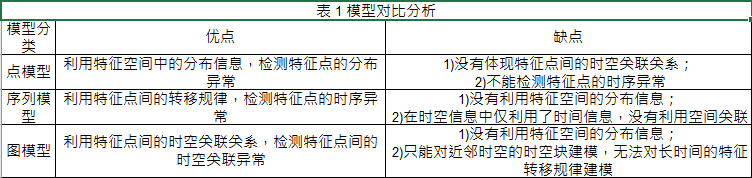
\includegraphics[width=1.0\textwidth]{compare1.png} 
\caption{模型对比分析} 
\protect\cite{qh2020}
\end{figure}
从 表 1 的对比分析可以发现,不同模型对时空信息的利用程度不同,且依据异常事件的不同属性检测异常。因此,不同模型在异常检测上具有互补性,可以通过将不同模型相结合来提升算法的异常检测效果。

\subsubsection{判别对比分析}
聚类判别与重构判别在各个发展阶段均得到了关注,本小节分析了它们在不同发展阶段的特点, 具体见 表 2。
\begin{figure}[H] 
\centering 
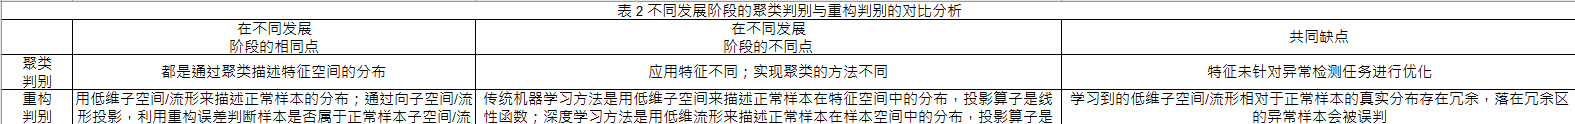
\includegraphics[width=1.0\textwidth]{compare2.png} 
\caption{判别对比分析} 
\protect\cite{qh2020}
\end{figure}

\bibliography{cites.bib}
\bibliographystyle{ieeetr}

\end{document}
% PyOD
% 开源,包含各种算法的详细文档和示例
% 支持高级模型,包括神经网络,深度学习和异常集合
% 使用Numba和joblib优化JIT(即时)和并行化的性能

% 以后在讲ISOMAP和LLE的时候提到如何使用KNN和最短路径算法等工具实现非欧空间到欧氏空间转化
% 明确代价函数是什么:是点距离的和啊!那么更新策略是什么?是找中心点啊!
% 不考虑时间复杂度,二分类,终极解决办法